\subsection{The Additive Gaussian Noise Model}
By assuming the measurements are corrupted by the additive Gaussian noise, the linear estimation model can be written as 
\begin{equation}
\mathbf{d} \sim \text{Gaussian}( \mathbf{A} \mathbf{h}_t),
\end{equation}
\vspace{0.3cm}
where\\
\begin{tabular}{l c l}
$\mathbf{d}$ &=& a vector of measurements,\\
$\mathbf{A}$ &=& a linear forward operator,\\
$\mathbf{h}_t$ &=& the true bathymetry (depth). 
\end{tabular}

\vspace{0.3cm}
\noindent Therefore, the Gaussian noise $\boldsymbol{\epsilon}$ corrupted measurements $\mathbf{d}$ with variance $\nu$ is given by 
$$
\mathbf{d} = \mathbf{A} \mathbf{h}_t + \boldsymbol{\epsilon}.
$$



\subsection{Bathymetric Inversion Method}

As a beginning to approximate the topographic heights of the sea-floor,  we consider the following least-squares minimization problem,
\begin{equation}\label{LS}
\mathbf{\hat{h}}= \underset{\mathbf{h} \in \mathbb{R}^n}{\arg \min} \ \ f(\mathbf{h}) = \|  \mathbf{A}\mathbf{h} -  \mathbf{d} \|_2^2,
\end{equation}
where we minimize the data misfit between the forward predictions and the measurements in least-squares sense. 
This least-squares minimization problem \eqref{LS} can be solved using the following  MATLAB functions:
\begin{itemize}
\item[(1)]  Nonnegative least-squares method:  \verb|lsqnonneg(A,b)|. This Matlab function uses the algorithm so called \textit{active-set} and note that it requires matrix $\mathbf{A}$ explicitly. Residual norm error for the sample dummy data set  with $\nu = 0.1$ is $8.88 \times 10^{-26}$ (see Fig. \ref{nonLS_fig}).   \\

\begin{figure}[H]
\center
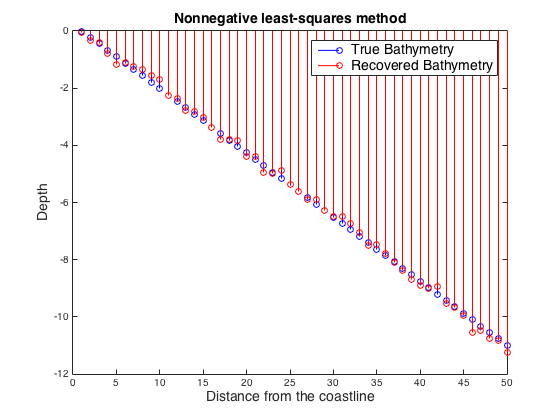
\includegraphics[scale=0.6]{img/NonLS_linear.png} 
\caption{Nonnegative least-squares method reconstruction of depth $\mathbf{h}$ using sample data.}
\label{nonLS_fig}
\end{figure}
\item[(2)]  Trust-Region-Reflective method:  \verb|lsqnonlin(f)|. Residual norm error for the sample dummy data set  with $\nu = 0.1$ is $4.32 \times 10^{-10}$. 
\begin{figure}[H]
\center
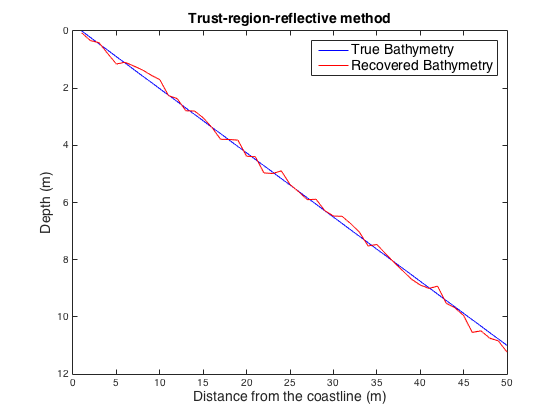
\includegraphics[scale=0.6]{img/trust_region_linear.png} 
\caption{Trust-Region-Reflective method reconstruction of depth $\mathbf{h}$ using sample data.}
\label{trust_region_fig}
\end{figure}
\item[(3)]  Levenberg-Marquardt (LM) method:  \verb|lsqnonlin(f, 'Algorithm', 'levenberg-marquardt')|. Residual norm error for the sample dummy data set  with $\nu = 0.1$ is $6.39 \times 10^{-13}$. The Levenberg-Marquardt algorithm does not handle bound constraints. 
\begin{figure}[H]
\center
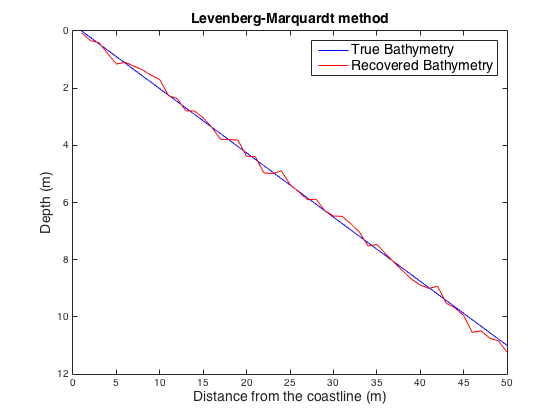
\includegraphics[scale=0.6]{img/LM_linear.png} 
\caption{Levenberg-Marquardt (LM) method reconstruction of depth $\mathbf{h}$ using sample data.}
\label{LM_fig}
\end{figure}
\item[(4)]  fmincon method:  \verb|fmincon(f)|. Residual norm error for the sample dummy data set  with $\nu = 0.1$ is $1.29$. 
\begin{figure}[H]
\center
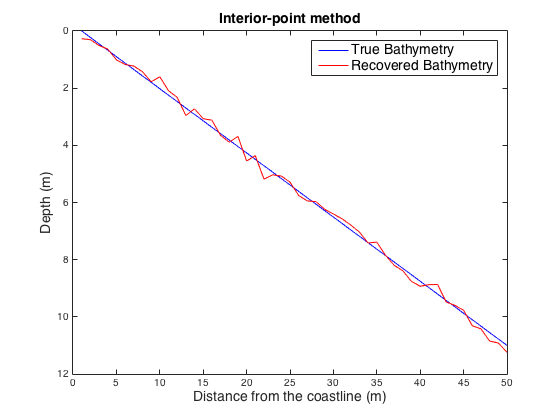
\includegraphics[scale=0.6]{img/fmincon_linear.png} 
\caption{fmincon method reconstruction of depth $\mathbf{h}$ using sample data.}
\label{LM_fig}
\end{figure}
\end{itemize}
%Challenges: What is the dimension of the $\mathbf{A}$? Is this a underdetermined or overdetermined system? If so, we have to consider the Tikhonov regularization,
If the inverse problem in \eqref{LS} is ill-posed, we have to consider a regularized version of it. If we have some prior estimate for the $\mathbf{h}$, i.e., $\mathbf{h}_p$, then the Tikhonov regularized solution with a prior information can be written as
$$
\mathbf{\hat{h}} = \underset{\mathbf{h} \in \mathbb{R}^n}{\arg \min} \|  \mathbf{A}\mathbf{h} -  \mathbf{d} \|_2^2  +  \alpha \| \mathbf{h} -  \mathbf{h}_p\|_2^2,
$$
where $\alpha$ is a regularization parameter $(>0)$. To test this method, Tikhonov method is implemented and test with sample data set with $\nu = 0.2$. This reconstruction of depth has 0.038 residual norm error. In order to run this \verb|tikhonov| Matlab function, matrix $\mathbf{A}$ should be explicitly known.

\begin{center}
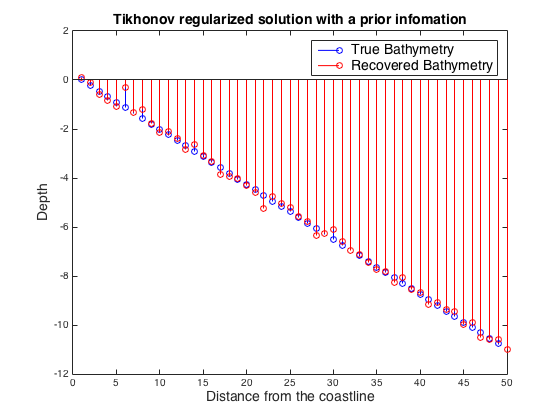
\includegraphics[scale=0.6]{img/Tikhnove_reg.png} 
\end{center}

Reference: I found a MATLAB package for analysis and solution of discrete ill-posed problems, which is available in http://www2.imm.dtu.dk/~pcha/Regutools/\\

\subsection{Help}

LSQR method: $\hat{\Psi}$ = lsqr(A,d,tol,maxit) it attempts to solve the least squares solution x that minimizes norm$(\mathbf{d}-\mathbf{A\Psi})$ Note that $\mathbf{A}$ need not be square.


Conjugate gradients: $\hat{\Psi}$ = cgs(A,b) attempts to solve the system of linear equations $\mathbf{A}\mathbf{\Psi} -  \mathbf{d}$ for $\Psi$.

